\documentclass[12pt]{article}
\usepackage[a4paper, total={15cm,24cm}]{geometry}
\usepackage{titlesec}
\usepackage{graphicx}
\usepackage{float}      % 設定圖片位置
\usepackage{hyperref}
\usepackage{fontspec}   % 加這個就可以設定字體
\usepackage{xeCJK}      % 讓中英文字體分開設置
\usepackage{comment}
\setCJKmainfont{宋體-繁}
\setmainfont{Times New Roman}
\renewcommand{\baselinestretch}{1.5}

\title{The Impact of Tariffs on Price and Welfare: \\ Literature Reviews and Future Research Plans}
\author{Ming-Chieh, Chang\thanks{Department of Economics, National Taiwan University}}

\begin{document}

\maketitle

\begin{abstract}
This report broadly reviews the role of tariffs in price, welfare, distributional effects, and productivity effects, especially on the tariffs of US-China trade war.
With recent monumental papers, I include both theoritical and empirical analyses on the effect of tariffs to see how tariffs affect consumers, producers, and even policymakers.
Also, I emphasize the importance of the role international trade plays in Taiwanese economic development, and give the structure for my further research plans.
\end{abstract}

\section{Introduction}
\label{sec:intro}
As the US-China trade war largely affected the whole world since 2018, 
trade economists have made lots of effort trying to find out the true causal impact of those tariff enacted. 
From applying econometric methods to constructing quantitative models, 
the change of price, welfare, or even more conceptual economic issues such as distributional effect and productivity were measured in many ways.
As an export-oriented country, international trade plays an important role in economic development of Taiwan.
Therefore, in this review I will explain some monumental papers about the impact of tariffs, 
especially those regarding to the US-China trade war, and discuss how Taiwan may be affected by the trade war through various possible channels.

\section{Price and Basic Welfare Impact}
\label{sec:price, welfare}
An conventional method to evaluate the effects of tariffs on price and welfare is a graph with an export supply curve intersecting with an import demand curve. \cite{amiti2019impact}
As shown in figure \ref{tariff_welfare}, when an ad valorem tariff is imposed, the export supply curve shifts upward. 
As a result, price raises from $P_2$ to $P_1$, where exporting suppliers bear the burden rectangle C and importing consumers bear the burden rectangle A 
(deadweight loss B + D in this general case).
However, when the export supply is perfectly elastic as presented in figure \ref{tariff_welfare_flat}, 
tariff burdens will all fall on importing consumers since there is only rectangle A, and rectangle C does not exist anymore 
(deadweight loss B in this perfectly elastic export supply case).
Now, the relationship between export supply elasticity, price, and welfare effect is clear. 
That is, we can estimate how much of the tariff burdens fall on importing consumers and how much on exporting producers by estimating the elasticity of the export supply curve.

Under this simple framework of estimation, Amiti et al. (2019) \cite{amiti2019impact}, Waugh (2019) \cite{waugh2019consumption}, Fajgelbaum et al. (2020) \cite{fajgelbaum2020return}, 
and many other papers all found that in the US-China trade war, the elsticity of the export supply is almost perfectly elastic 
(or more formally speaking, the null hypothesis that the export supply had a infinite elasticity could not be rejected). 
This surprising finding in turn implied that all tariff burdens in the trade war were borne by importing consumers, no matter which country they lived. 
Producers, on the other hand, gained some welfare increase by selling more products to consumers that previously bought imported products and some mark-ups in selling price.
Hence a natural question here is, summing up all consumers and producers, how much net welfare a country (e.g. the U.S.) gained or lost in the trade war?
To answer this question, Fajgelbaum et al. (2020) \cite{fajgelbaum2020return} used a three-tier CES demand system to construct a general equilibrium analysis. 
It turned out that the net welfare effect was relatively small and was not statitically significantly different from 0. 
The net zero result thus prompts us to turn our analysis to the distributional effect of tariffs since there were undoubtedly, winners and losers in international trade, 
which might also indirectly inform us what is the main rationale behind the trade war.

\begin{figure}[H]
    \centering
    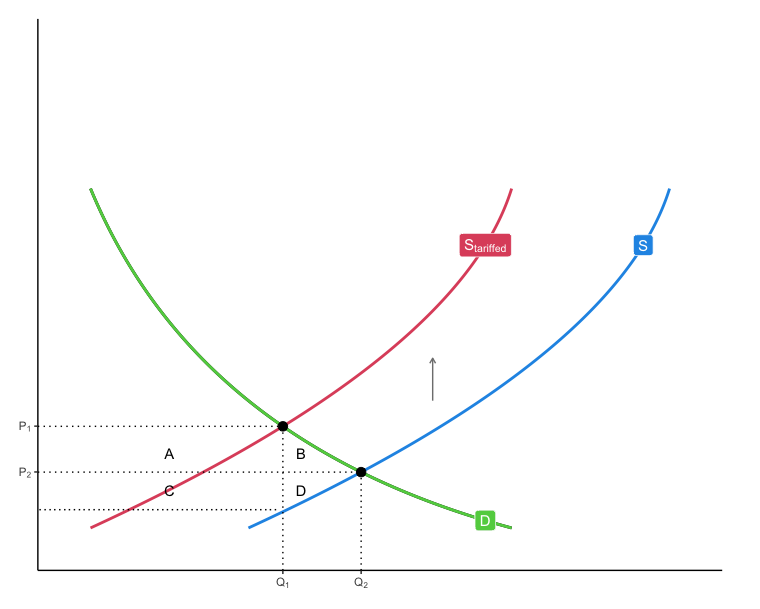
\includegraphics[width = 0.6\textwidth]{tariff_welfare.png}
    \caption{Impact of a Tariff on Price and Welfare}
    {\footnotesize X-axis: imported quantity, Y-axis: price, \\ 
    $S, S_{tariffed}$ are the export supply curves and $D$ is import demand curve \par}
    \label{tariff_welfare}
\end{figure}

\begin{figure}[H]
    \centering
    \includegraphics[width = 0.6\textwidth]{tariff_welfare_flat.png}
    \caption{Impact of a Tariff on Price and Welfare with Perfectly Elastic Export Supply}
    {\footnotesize X-axis: imported quantity, Y-axis: price, \\ 
    $S, S_{tariffed}$ are the export supply curves and $D$ is import demand curve \par}
    \label{tariff_welfare_flat}
\end{figure}

\clearpage

\section{Distributional Effects and Rationales of the Trade War}
\label{sec:distributional}
Winners (producers) and losers (consumers) are clear from discussions performed in the previous section.
For further understanding of the distributional effects of the US-China trade war, we need to figure out which industries those winning producers belonged to, and which groups of consumers suffered the most from the tariffs. 
Unfortunately, for the first question, since there was a lack of variation in tariffs across industries, 
we could hardly observe any analyzable differential tariff protection across producers. Hence there are few analyses for producers across industries. 
In contrast, we have much more information on the consumers. 
From the general equilibrium in Fajgelbaum et al. (2020) \cite{fajgelbaum2020return}, 
though consumer welfare loss occured everywhere in the US, there were still some variations across counties. 
The reason of these variations was that different counties specialized in different industries, 
and different industries were retaliated by China (and other countries) to different degrees.
The general equilibrium analysis implied that the consumer welfare losses were highly concentrated in the Midwestern Plains since they were hit hardest by retaliatory tariffs.
Furthermore, combined with the voting patterns in 2016 presidential election, 
they found that the rationale behind the US-China trade war might probably lie in the competition of attracting pivotal voters since those politically competitive counties were the most protected by US tariffs.
The finding here was consistent to the logic of majority voting.
Nevertheless, this evidence is still relatively suggestive and requires more formal econometric analyses to be further verified.

\section{Productivity Effects from Tariffs}
\label{sec:productivity}
The effect of trade on firm-level productivity selection has been broadly discussed since Melitz (2003) \cite{melitz2003impact} proposed a heterogeneous firm model in trade.
As summarized in Melitz and Trefler (2012) \cite{melitz2012gains}, in the heterogeneous firm model, trade selects firms with higher productivity to expand to larger scale, to gain more market share, and thus to improve market efficiency. 
This model was verified by Canadian data in this paper and other empirical evidence such as Amiti and Konings (2007) \cite{amiti2007trade}, using indonesia tariff data.
In this case, tariffs that block trades should have a negative impact on firm-level productivity growth. 

However, there is also another more traditional way to analyze the effect of protections (tariffs) on productivity, namely the learning-by-doing model presented in Krugman (1987) \cite{krugman1987narrow}. 
This model predicted that temporary protection on specific industries might help infant industries accrue productivity increase through learning-by-doing, which leads to long-term comparative advantage.
The point was verified by Juhasz (2018) \cite{juhasz2018temporary} with a rigorous causal analysis on Napolenic blockade.
In this sense, temporary tariffs may lead to a long-term positive productivity growth.

Two ways presented above to analyze impact of tariffs on productivity are not contradictory. 
In Melitz model, there are productivity gains "within" an industry through trade, so tariffs might hinder productivity growth.
On the other hand, the Krugman model presented the productivity change "between" industries, so tariffs might be beneficial for productivity in those protected industries.

Through the above discussions, we now suggest that tariffs in the US-China trade war may hinder some productivity gain within some protected industries, 
but those tariffs may also help some infant industries in the US avoid stringent competition from foreign companies and thus lead to long-term growth in productivity. 
Literatures about productivity effects on the US-China trade war now remains relatively small since it is more difficult to be estimated than welfare, 
so here we just simply point out two possible channels of how US-China trade could affect productivity. An accurate estimation would require more detailed analyses.

\section{Effects of the US-China Trade War on Taiwan}
\label{sec:Taiwan}
As we mentioned in section \ref{sec:intro}, an export-oriented economy like Taiwan was greatly affected by the US-China trade war.
To be more specific, high tariffs in the US against exports from China may be favorable for Taiwanese exporters in the short run, 
but loss incurred by Chinese consumers may reduce their ability to import products from Taiwan.
Therefore, the welfare effects of Taiwan are extremely complicated under trade shocks brought by the US-China trade war.
We need to first specify which channels affect Taiwanese economy the most, and in turn take suitable econometric methods to estimate them.
For example, if we hypothesize that the most important effect is the Taiwanese exporter gains from US high tariffs against Chinese exporters, 
we must claim the exogeniety of tariff change and perhaps use instrumental varuables to measure how much those Taiwanese exporters gain. 

In addition to the welfare effects, I am also interested in the connection between trade policy making and voting patterns in Taiwan during the US-China trade war, 
so I plan to conduct methods similar to Fajgelbaum et al. (2020) \cite{fajgelbaum2020return} to capture possible political considerations underlying current trade policies.
As for the productivity effects, due to the difficulties of measurement mentioned in section \ref{sec:productivity}, I will not put it as a priority of research topic but as a future extension. 

In conclusion, I plan to conduct research with issues around Taiwanese trade mentioned above step by step as my senior thesis, 
try to figure out the effect of US-China trade war on Taiwan, and analyze possible policy making rationales. 
Moreover, I hope these analyses can be helpful for future trade policy making, which should aim to help those sufferring from trade shocks in the short run.
On the other hand, in the long run, since trade policy could help promising infant industries grow as mentioned in section \ref{sec:productivity}, 
I hope to suggest what industries are worthy of protection by analyzing their potentials to grow. 
I believe these are important lessons that trade economists can provide for the society.


\bibliographystyle{plain}
\bibliography{trade_review_ref}

\end{document}